\mychapter{TD2}
\label{Cap:TD2}

\section{Diagramme UC de haut niveau}
\begin{figure}[h]
    \centering
    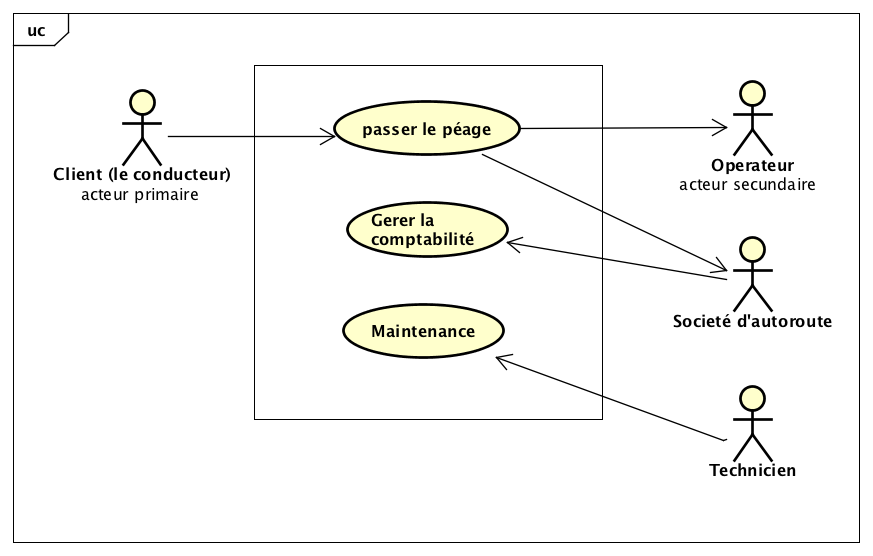
\includegraphics[scale=0.55]{images/hautNiveau.png}
    \caption{Diagramme de haut niveau - Passer le péage}
    \label{fig:my_label}
\end{figure}
\newpage
\section{Scenários Cockburn - Passer le péage}\label{sec:passer}
    \textbf{Cas d'utilisation:} Passer le péage
    
    \textbf{Acteur primaire (initiateur):} Conducteur
    
    \textbf{Acteur support:} -
    
    \textbf{Pré-condition: } nécessite que la voie soit ouverte.
    
    \textbf{Post-condition: }   la voie redevient disponible(ouverte et libre) pour un prochain usager.
    
    \textbf{Scenario primaire: } \\
    \textbf{1.} L’usager rentre dans la voie d’autoroute. \\
    \textbf{2.} L’usager paie le passage (\ref{subsec:paie})\\
    \textbf{3.} L’usager passe.
    
    \textbf{Variantes}\\
    \textbf{3a.} L'usager ne passe pas : la barrière reste ouverte en attendant la sortie de l’usager.

\section{Scenários Secundaries}
\subsection{Scenários Cockburn - Paie le passage} \label{subsec:paie}
\textbf{Cas d'utilisation:}

\textbf{Acteur primaire:}Paie le passage Conducteur

\textbf{Acteur support:} le poste de surveillance et opérateur humain(si le borne est manuelle)

\textbf{Pré-condition: } La boucle au sol détermine la présence du véhicule
 
\textbf{Post-condition: } 

\textbf{Scenario primaire: } \\
    \textbf{1.} Paier pour carte bancaire\\
    \textbf{2.} Paier avec argent\\
    \textbf{3.} Paier avec cart abonnement\\

\textbf{Variantes:}\\
    \textbf{2a.} Verifier pièces %Se algo é feito automatico eu devo escrever? ps2: se é so feito pela borne automatique, como escrevo condicao? 
\subsection{Scenários Cockburn} \label{subsec:}
\textbf{Cas d'utilisation:}

\textbf{Acteur primaire:}

\textbf{Acteur support:}

\textbf{Pré-condition: } 
 
\textbf{Post-condition: } 

\textbf{Scenario primaire: } \\
    \textbf{1.} \\
    \textbf{2.} \\
    \textbf{3.}

\textbf{Variantes:}\\
    \textbf{2a.} 
\newpage
\section*{Diagrammé UC détaillés}
\begin{figure}[h]
    \centering
    %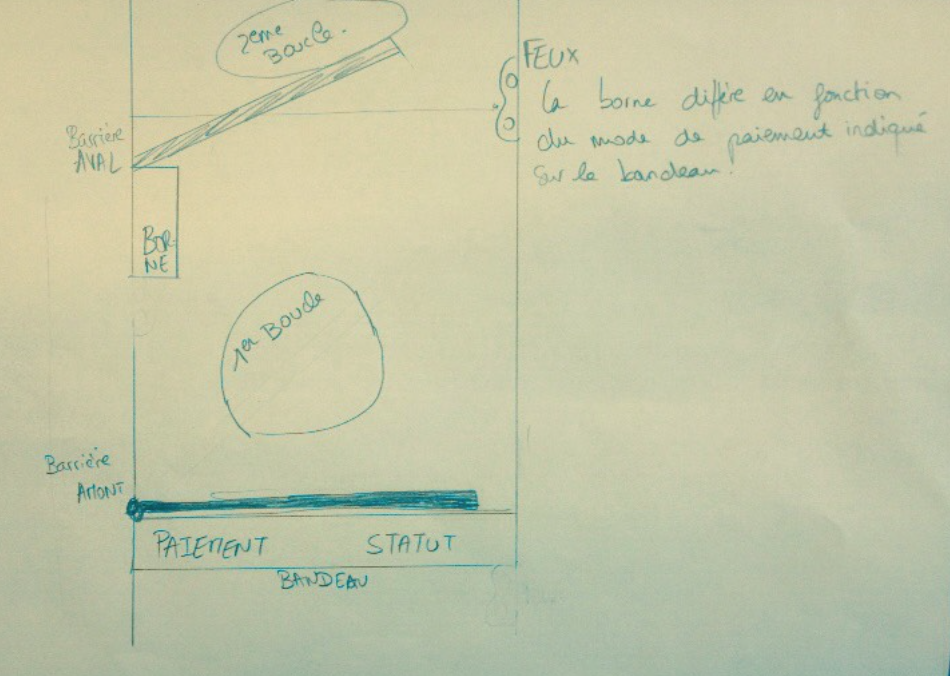
\includegraphics[scale=0.9]{a.png}
    \caption{Diagrammé UC détaillés - passage}
    \label{fig:my_label}
\end{figure}